%\section{}
\subsection{Topologies des réseaux}
Maintenant que nous connaissons le matériel nécessaire pour établir une connexion, nous pouvons voir les différentes manières possible de les connecter entre-eux. La façon dont les appareils sont connectés entre-eux est appelée \textbf{topologie}. On peut différencier deux types de topologies.

\UPSTIdefinition{
  La \textbf{topologie physique} désigne la configuration spatiale du réseau. C'est la façon dont les organes sont connectés \textbf{physiquement}.
}
\UPSTIdefinition{
  La \textbf{topologie logique} désigne quant à elle la manière dont les données transitent dans les câbles.
}


%\begin{figure}[h!t]
%  \centering
%  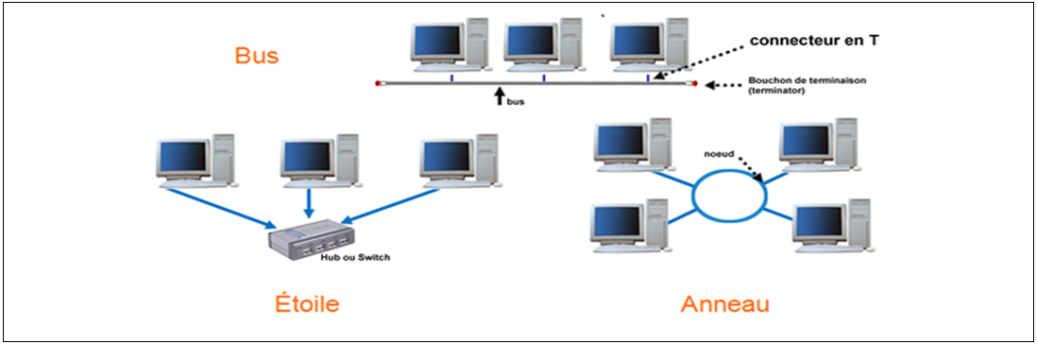
\includegraphics[width=.7\textwidth]{images/topologies/reseau_topologies}
%  \caption{Trois exemples de topologies de réseau.}
%  \label{fig:res_topo}
%\end{figure}
\subsubsection{Topologie en bus}
\begin{figure}[h!]
  \centering
  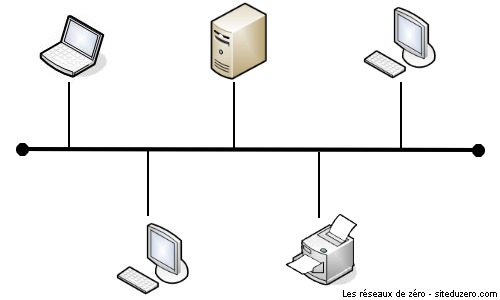
\includegraphics[width=.4\textwidth]{images/topologies/topologieBus}
  \caption{Topologie en BUS}
  \label{fig:topoBus}
\end{figure}
Une topologie en bus (Figure~\ref{fig:topoBus}) est l'organisation la plus simple d'un réseau. Dans une topologie en bus tous les ordinateurs sont reliés à une même ligne de transmission par l'intermédiaire d'un seul câble. Le mot "bus" désigne la ligne physique qui relie les machines du réseau.

Cette topologie a pour avantages d'être {facile à mettre en oeuvre} et de fonctionner facilement, par contre elle est extrêmement {vulnérable} étant donné que si l'une des connexions est défectueuse, c'est l'ensemble du réseau qui est affecté.

Cette topologie est obsolète dans les réseaux de données mais couramment utilisé dans les réseaux de terrain (automates industriels ou voitures par exemple).

\subsubsection{Topologie en anneau}

Dans un réseau en topologie en anneau, les ordinateurs sont reliés sur une bouble. On peut le voir comme un réseau en bus dont on a relié les extrémités. Comme pour le réseau en BUS, les composants ne peuvent pas communiquer en même temps car cela créerait une collision de données. Dans une topologie en anneau, les appareils communiquent chacun leur tour en échangeant un jeton (\textit{token})

En réalité les ordinateurs d'un réseau en topologie anneau ne sont pas reliés en boucle, mais sont reliés à un répartiteur (appelé MAU, Multistation Access Unit) qui gère la communication entre les différents composants.

\subsubsection{Topologie en étoile}
\begin{figure}[h!]
  \centering
  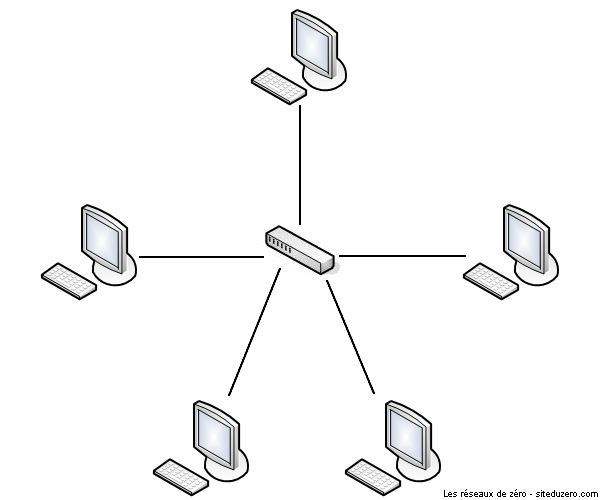
\includegraphics[width=.4\textwidth]{images/topologies/topologieEtoile}
  \caption{Topologie en étoile}
  \label{fig:topoEtoile}
\end{figure}
Dans une topologie en étoile (Figure~\ref{fig:topoEtoile}), les ordinateurs du réseau sont reliés à un noeud central. Chaque membre du réseau communique avec le noeud central au travers de sa propre connexion. Le noeud central fait le lien

Contrairement aux réseaux construits sur une topologie en bus, les réseaux suivant une topologie en étoile sont beaucoup moins vulnérables car on peut aisément retirer une des connexions en la débranchant du commutateur sans pour autant paralyser le reste du réseau.

\subsubsection{Topologie maillée}
\begin{figure}[h!]
  \centering
  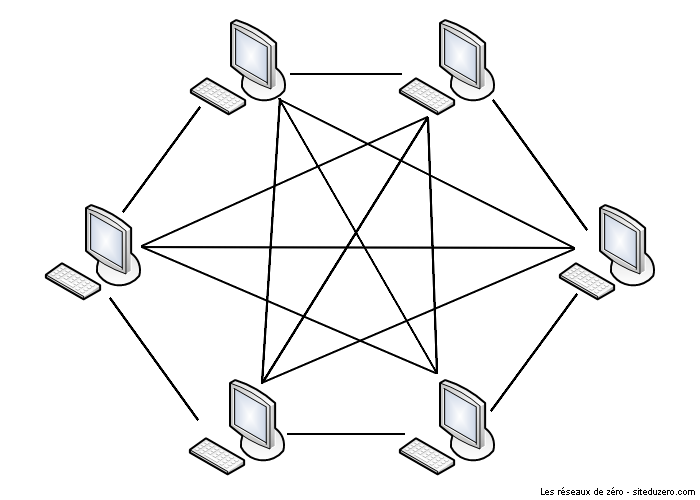
\includegraphics[width=.4\textwidth]{images/topologies/topologieMaillee}
  \caption{Topologie maillée}
  \label{fig:topoMaillee}
\end{figure}

Il s'agit de la topologie la plus robuste car tous les éléments sont connectés à tous les autres (Figure~\ref{fig:topoMaillee}). Chaque élément peut donc communiquer avec n'importe quel autre élément en utilisant la connexion propre. L'avantage d'une topologie maillée est sa robustesse aux pannes de raccordement. En effet, si le lien entre deux éléments est défectueux, cela n'aura une influence que sur la communication entre deux éléments. Les autres connexions sont toujours possibles. En passant par un intermédiaire, les deux éléments concernés peuvent d'ailleurs toujours communiquer.

En revanche, ce type de réseau impose un nombre de connexion considérable. Ce nombre est de $\frac{n(n-1)}{2}$ connexions, avec $n$ le nombre d'éléments connectés. Sur la Figure~\ref{fig:topoMaillee}, 6 éléments sont connectés, nécessitant $\frac{6 \times 5}{2} = 15$ câbles. Le calcul pour une institution ayant 500 machines donne alors un nombre de connexion de \num{124700}... C'est une architecture réseau qui convient donc dans des cas précis où la robustesse est primordiale et où la taille du réseau est suffisamment petite.
